\subsection{Quality of Service Metrics}

1 second live measurements from another thread

\begin{figure*}
  \centering
  \begin{subfigure}[b]{0.5\textwidth}
    \centering
    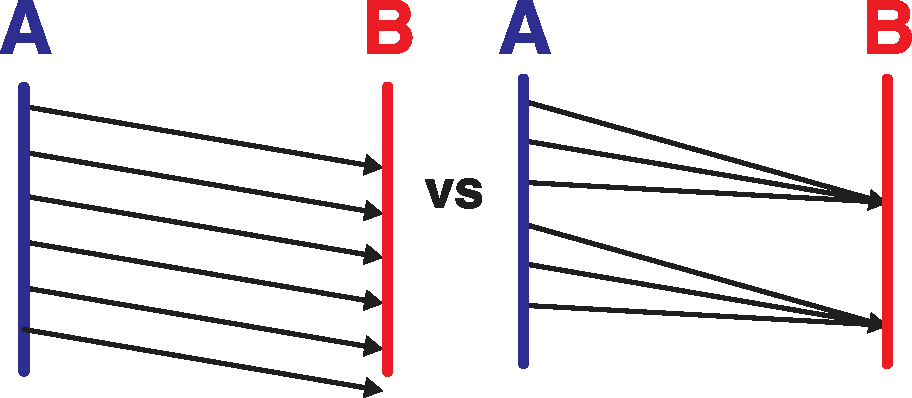
\includegraphics[width=\linewidth]{img/quality-of-service-metric-definitions/clumpiness.pdf}
    \caption{Clumpiness}
    \label{fig:quality-of-service-metric-definitions-clumpiness}
  \end{subfigure}%
  \begin{subfigure}[b]{0.5\textwidth}
    \centering
    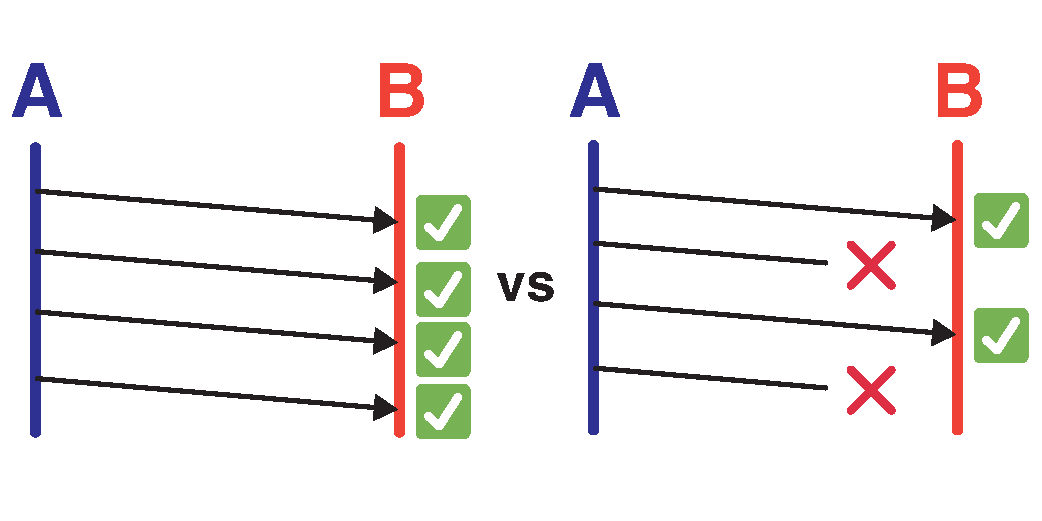
\includegraphics[width=\linewidth]{img/quality-of-service-metric-definitions/delivery-failure-rate.pdf}
    \caption{Delivery Failure Rate}
    \label{fig:quality-of-service-metric-definitions-delivery-failure-rate}
  \end{subfigure}
  \begin{subfigure}[b]{0.5\textwidth}
    \centering
    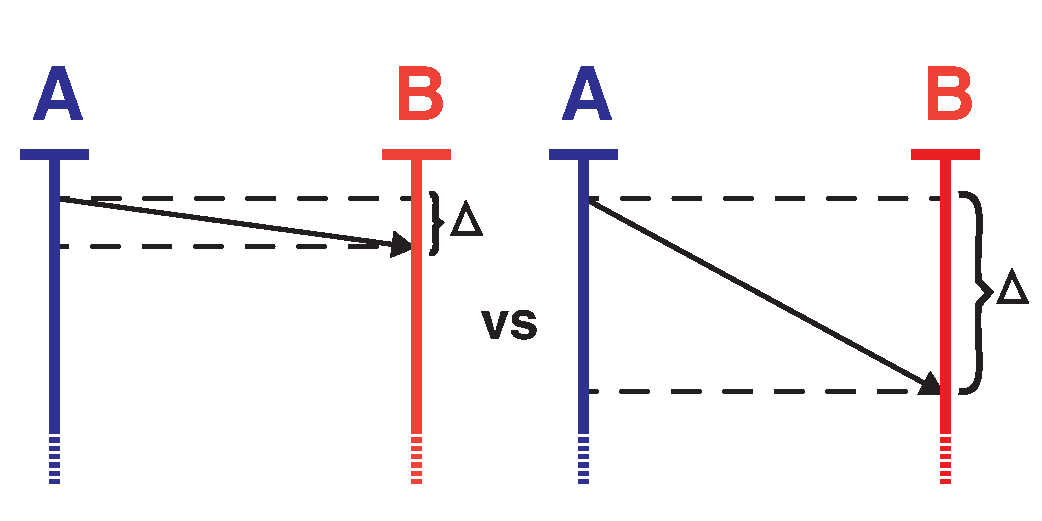
\includegraphics[width=\linewidth]{img/quality-of-service-metric-definitions/latency.pdf}
    \caption{Latency}
    \label{fig:quality-of-service-metric-definitions-latency}
  \end{subfigure}%
  \begin{subfigure}[b]{0.5\textwidth}
    \centering
    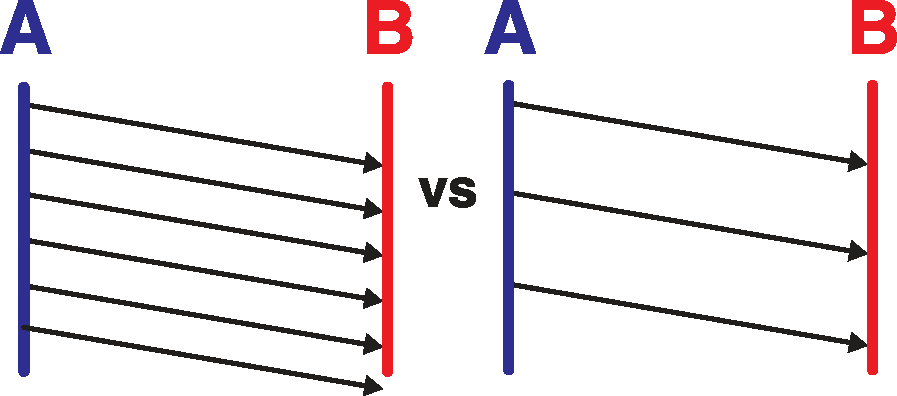
\includegraphics[width=\linewidth]{img/quality-of-service-metric-definitions/simstep-period.pdf}
    \caption{Simstep Period}
    \label{fig:quality-of-service-metric-definitions-simstep-period}
  \end{subfigure}%
  \caption{
  Quality of service metrics.
  Each illustration is a space-time diagram, with $A$ and $B$ representing independent processes.
  The vertical axis depicts the passage of time, from top to bottom.
  Solid black arrows represent message delivery.
  The left panel of each metric's diagram depicts a scenario with a lower (``better'') value for that metric compared to the right panel, which depicts a higher (``worse'') value for that metric.
  }
  \label{fig:quality-of-service-metric-definitions}
\end{figure*}


\subsubsection{Latency}

Simsteps and walltime.

To measure simstep latency, we round counted trip messages.
Messages between elements were tagged with a counter that.
Between inlet and outlet node pairs

\begin{itemize}
  \item latency (simsteps)
    - \verb|(df['Num Puts Attempted'] - 1) / df['Num Round Trip Touches Inlet']|
  \item latency (walltime)
    - \verb|df['Latency Simsteps Inlet'] * df['Simstep Period Inlet (s)']|
  \item delivery clumpiness
    - \verb|1.0 - df_snapshot_diffs['Num Pulls That Were Laden Immediately'] / df_snapshot_diffs[['Net Flux Through Duct', 'Num Pulls Attempted']].min(axis=1)|
  \item delivery failure rate
    - \verb|message sends attempted / messages delivered|
  \item simstep period (walltime)
    - \verb|df_snapshot_diffs['Inlet-Nanoseconds Elapsed'] / df_snapshot_diffs['Num Puts Attempted']|
\end{itemize}

How do we calculate each of these?

Inlet vs Outlet
